\section{Plopzilla Photo Trip}

\margininbox{Plopzilla}{
     \begin{itemize}
    \item Jarvist Frost
    \item Paul Hutton
    \item Andrew Jurd
    \end{itemize}}{\explo}

Andy's last trip; so it had to be \passage{Plopzilla}.

Set off with a Daren drum of gear, with Paul in the lead and Andy
bringing up the rear (Ooh-err!). Took a few firefly digital shots coming
up into \passage{Hotline}. Seems to be lots off the lower \passage{M16}
entrance series, such as pitches into \passage{Lost City}, etc.

More photos on the newly sexy \passage{Gladiators} rigging, then shot off up
\passage{Faulty Towers}. Popped into \passage{NCB}; Andy conned us into
pissing down \passage{Silos}:- ``Don't piss in the main passage, climb down
there but no further than the first bolt!''


\begin{marginfigure}
\checkoddpage \ifoddpage \forcerectofloat \else \forceversofloat \fi
\centering
 \frame{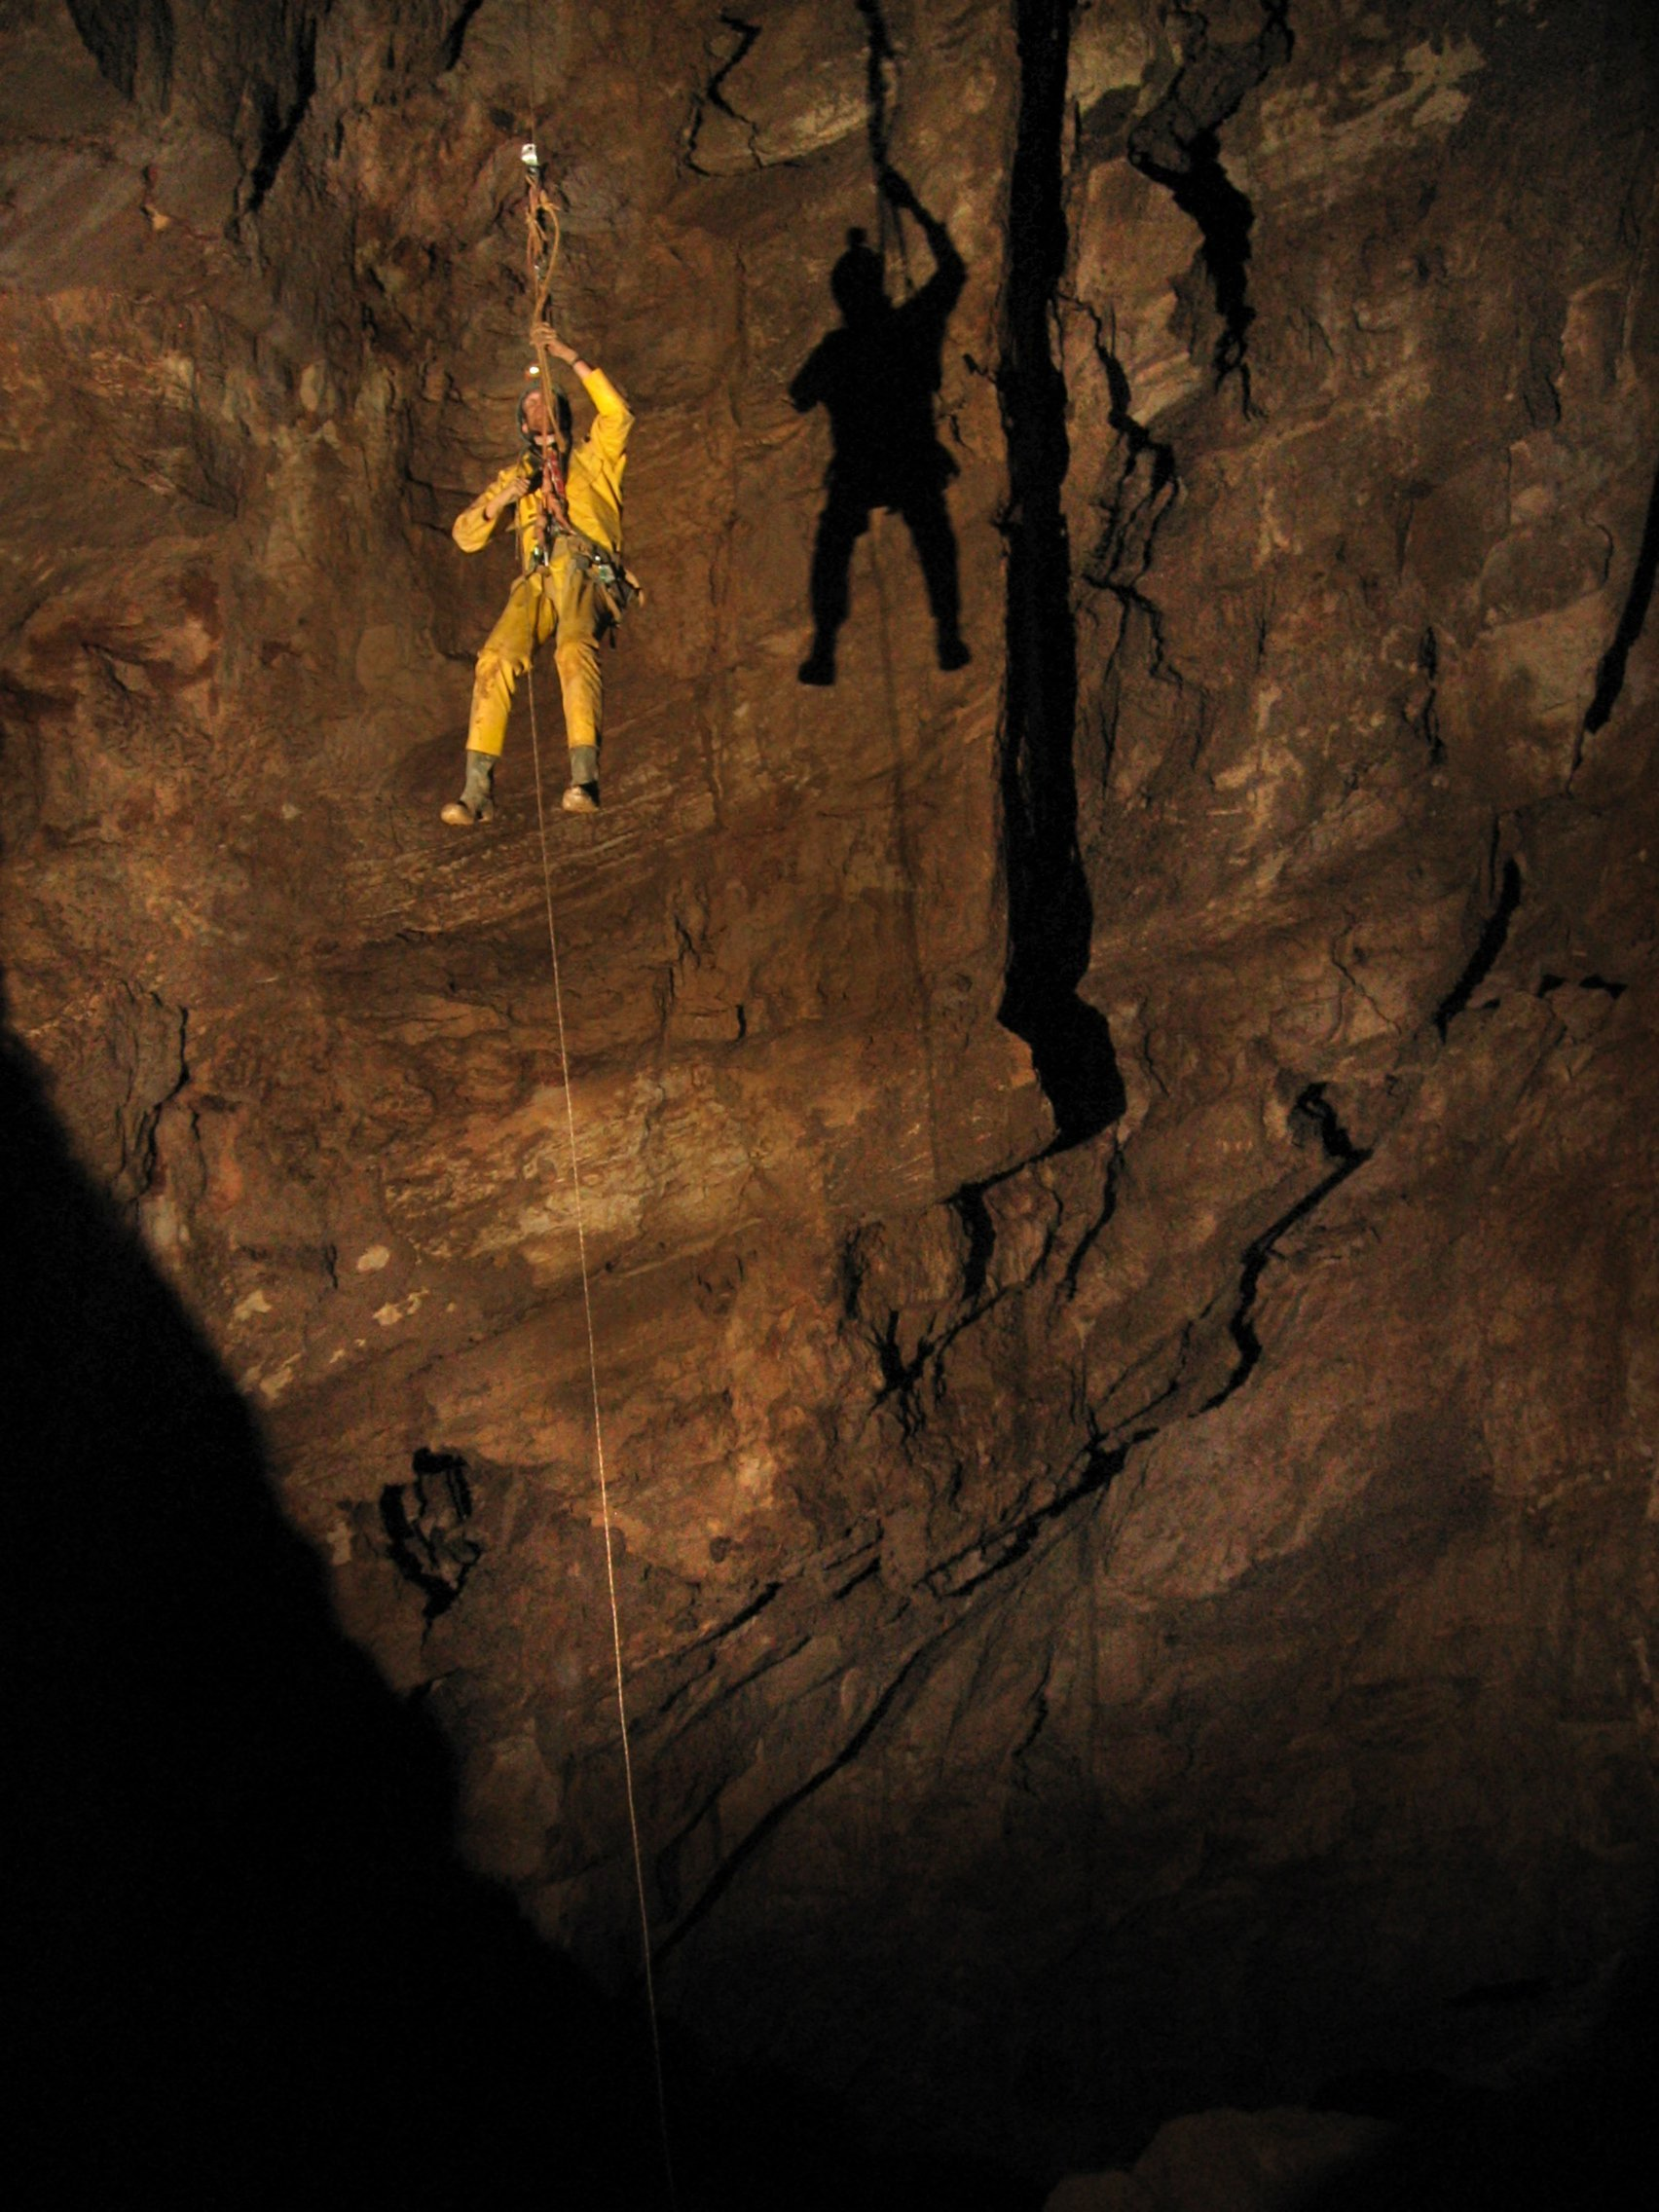
\includegraphics[width=\linewidth]{2008/Plopzilla_photo_trip/Jarvist Frost - canon a520 -plopzilla - andy 9mm knot pass b--orig.jpg}} 
 \caption{\protect\passage{Plopzilla} knot pass. \pic{Jarvist Frost}}
 \label{knotpass plopzilla}
\end{marginfigure}


Rerigged traverse in \passage{NCB} (more photos!), then to the main game:
\passage{Plopzilla}. We had a plan, I asbeiled down with gear \& scrambled
up a slope. Pitch head was `interesting' (clip in cows, push through
squeeze and swing out above the 105 m drop hoping cows were still in).
Rebelays were `interesting' (so tight, one had to climb above belay to
derig descender). Knot change `exciting' (knot a `Rik Special' - 9 mm
below super slippery). Gear down there `intriguing'
\sidenote{this explains where all the rope went; 90 m of 11 mm, 90 m of 9 mm and 1 tacklesac}.

We tried our best on 2 attempts at filming exploration, a few digital
pictures, and then dived into the boulder choke. Went down -30 m or so,
drips, went through a lot of very loose boulders then into bigger
stones, but with solid wall, lots of boulders. Many drips, no stream
hearable. Otherwise very similar to \passage{Jelly Chamber}. Got as far as
a loose committing climb into a large-ish chamber.

It goes, it really does. But I'm not going there. Stones rattled
$\approx$ 4 seconds.

Climbed ridge to corner and found another entry to choke. So we left \& derigged. Rope to \passage{Club Mig}. Sped out once gear stashed.
2hrs from bottom to \passage{Faulty Towers}.

\name{Jarvist Frost}


\begin{figure}
\checkoddpage \ifoddpage \forcerectofloat \else \forceversofloat \fi
\centering
 \frame{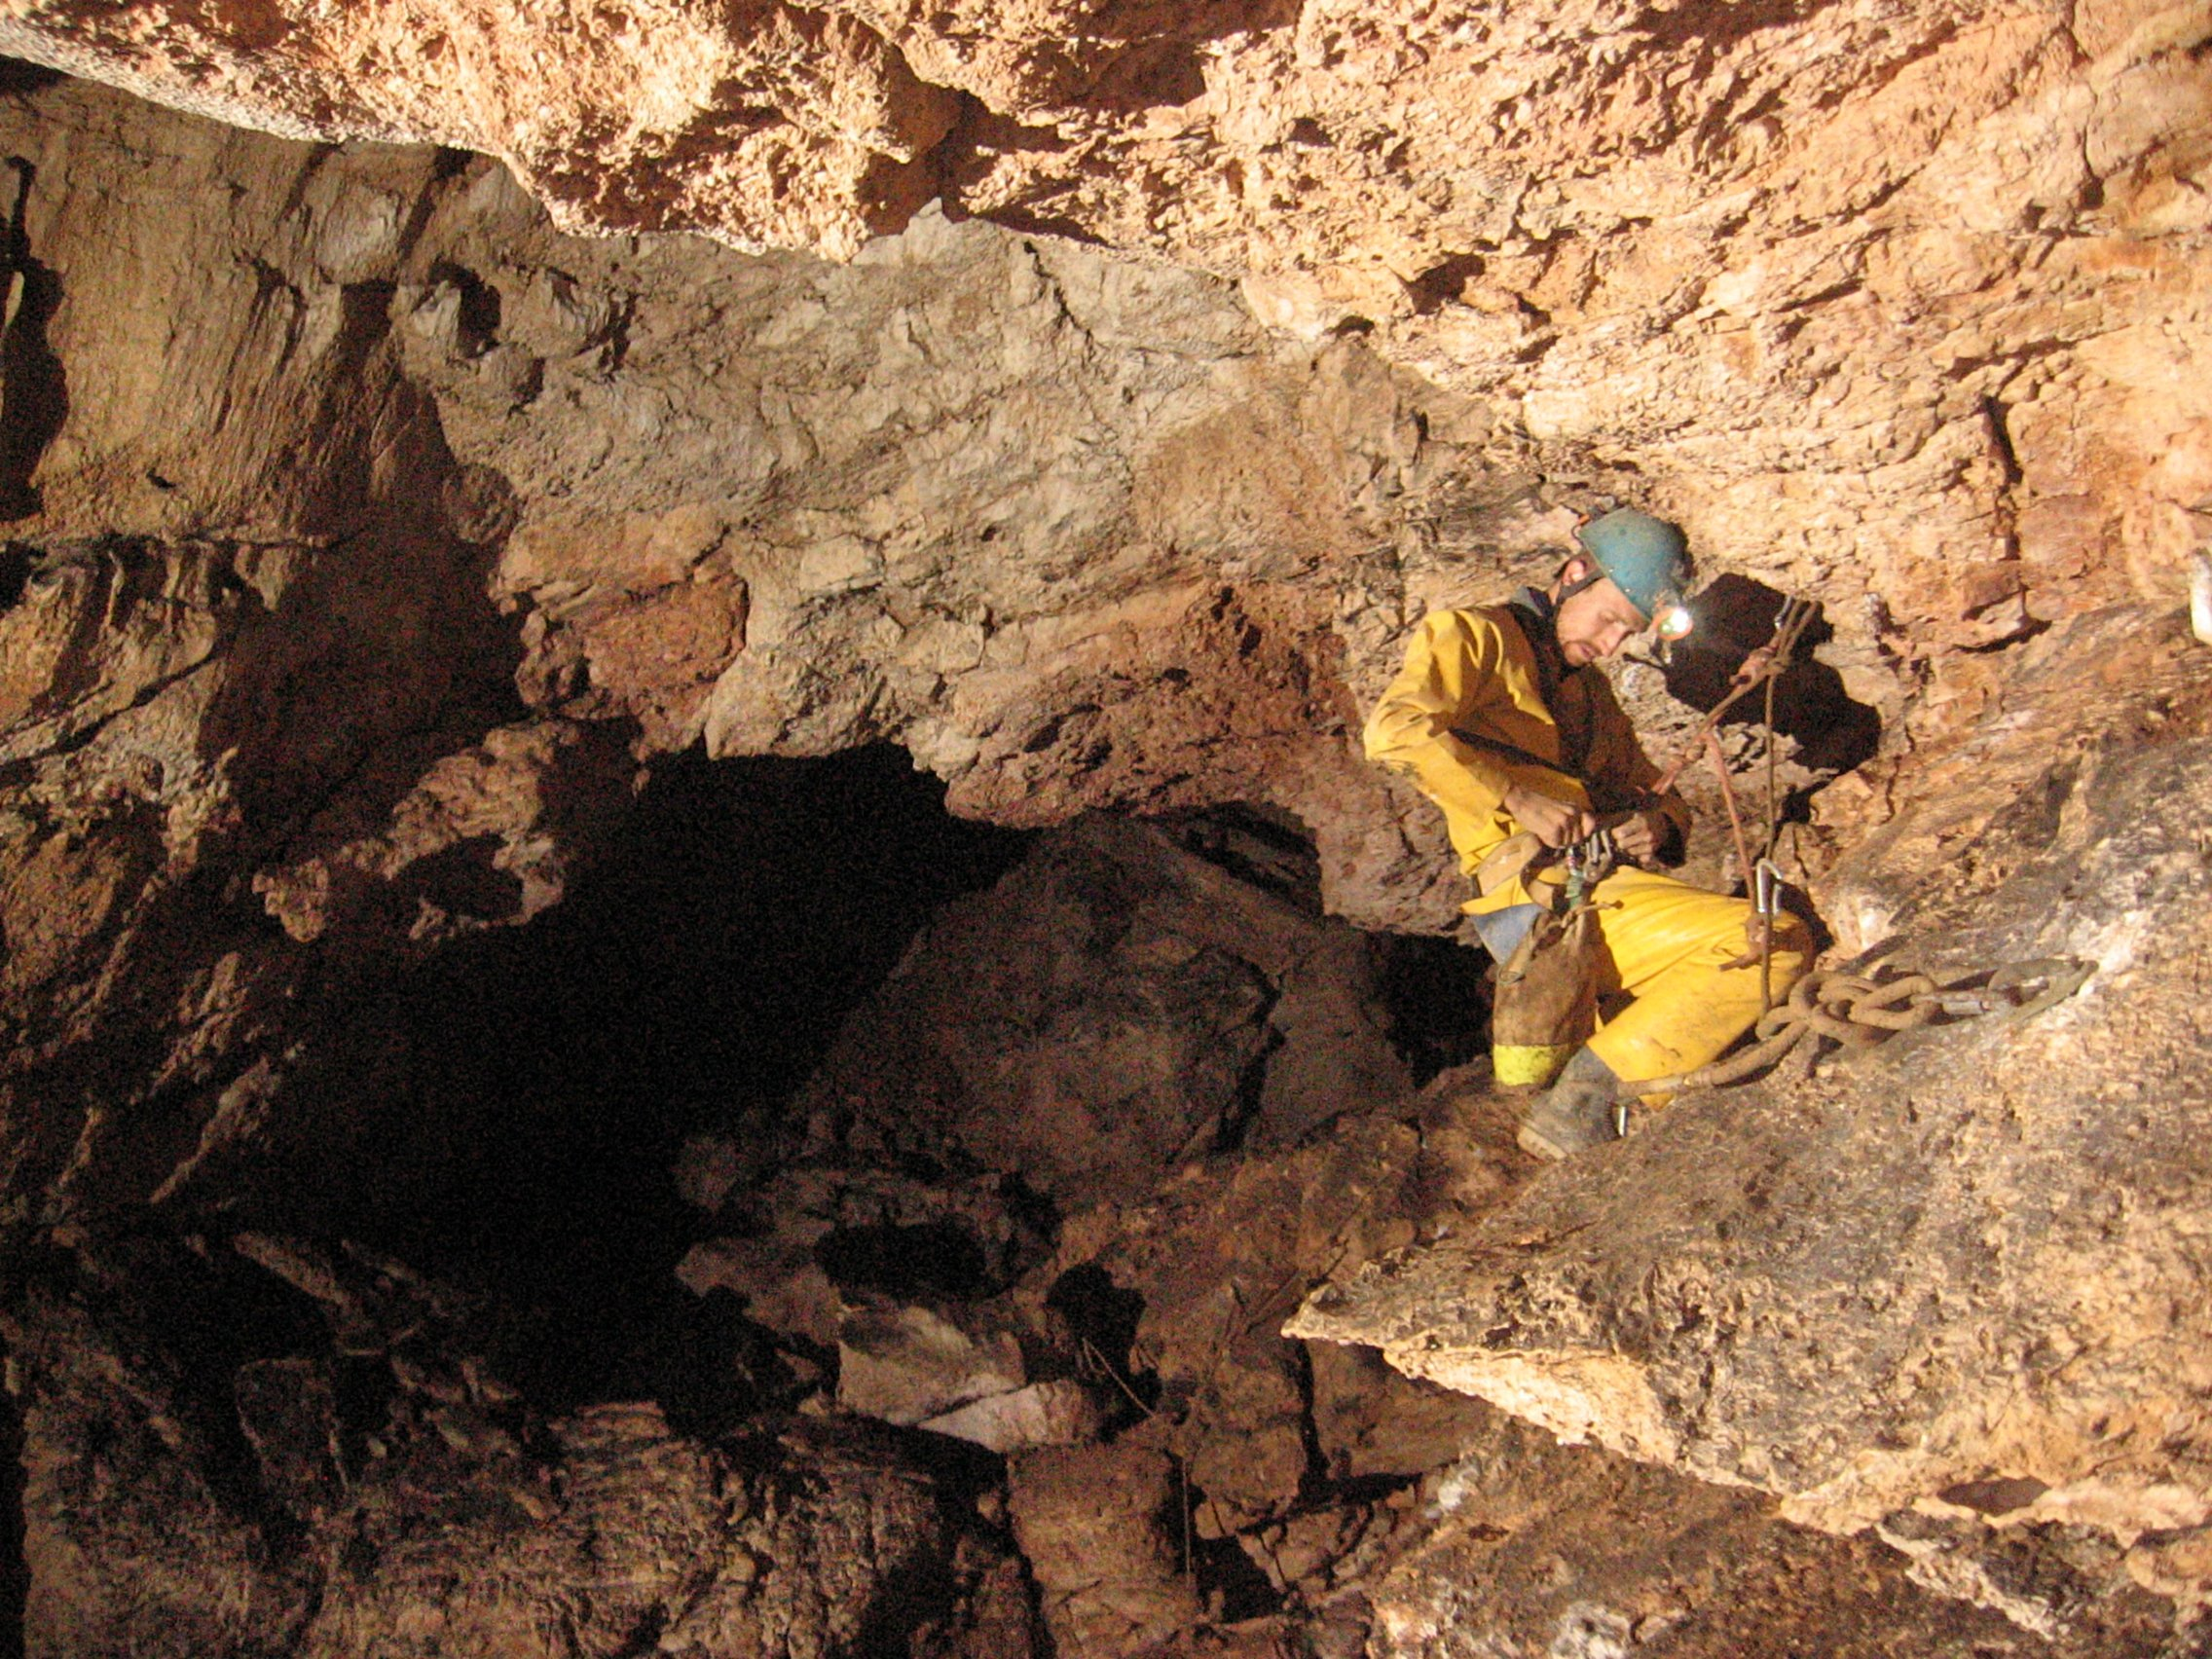
\includegraphics[width=\linewidth]{2008/Plopzilla_photo_trip/Jarvist Frost - canon a520 -ncb - andy fixing traverse to plopzilla closeup--orig.jpg}} 
 \caption{Andy Jurd altering the rigging on the traverse above \protect\passage{Plopzilla}. \pic{Jarvist Frost}}
 \label{Plopzilla traverse}
\end{figure}